% mainfile: ../../../../master.tex
\subsection{Migration of nucleic acids in agarose gel}
% The part of the label after the colon must match the file name. Otherwise,
% conditional compilation based on task labels does NOT work.
\label{task:20180130_cj1}
\tags{pcr,emp,dna,lab}
\authors{cj}
%\files{}
%\persons{}

\subsubsection{1\% Agarose gel preparation}

\begin{enumerate}
\item Measure with erlenmeyer 75~mL of 1\% agarose gel.\sidenote{The 1\% agarose gel is kept at 60\degree C in the gel room.}
\item Warm up the erlenmeyer for 15s in microwave: agarose will be more fluid and it will avoid bubbles when casting the gel
\item Add 3.75~\textmu L of SYBR Safe to the agarose while swirling \sidenote{SYBR Safe by Invitrogen, 10,000X in \gls{dmso}}
\item Cast the gel with the comb (for 20 wells)
\item Let the gel set for 20 min
\end{enumerate}

Just after the coffee break, my \gls{pcr} products are ready and waiting for me in the thermocycler at 4\degree C. 

\subsubsection{\gls{pcr} products preparation}

With a multichanel pipette:
\begin{itemize}
\item 5~\textmu L of each sample of \gls{pcr} product
\item 5~\textmu L of blue dye (bromothymol blue)
\item Tap gently tubes to mix up everything
\item Centrifuge briefly to bring all the liquid to the bottom
\end{itemize}

\subsubsection{Electrophoresis}

For this electrophoresis migration, we run:
\begin{itemize}
\item 9~\textmu L of each sample of \gls{pcr} products
\item 5~\textmu L of the 100~pb ladder
\end{itemize}

\begin{enumerate}
\item Place the agarose gel into the gel box (electrophoresis unit) containing TAE buffer
\item Load 5~\textmu L of molecular weight ladder into the first and last lane of the gel
\comment{I leave one empty well between the ladder and the samples.}
\item Load 9~\textmu L of each sample into the additional wells of the gel
\item Run for 45~min with the \gls{eps} 301 at 100~V, 400~mA
\comment{I usually leave the gel for 50 min, but I was too impatient.}
\item Visualize your \gls{dna} fragments with \gls{uv} lights
\end{enumerate}

\begin{figure}[H] % position of the figure 
    \centering
    \caption{Picture of 1\% agarose gel after 50 minute-long electrophoresis migration of \gls{pcr} products obtained with \gls{emp} primers and \gls{dna} extrated from surface seawater samples.}
    \label{fig:20180130_EMP_OneTaq}
    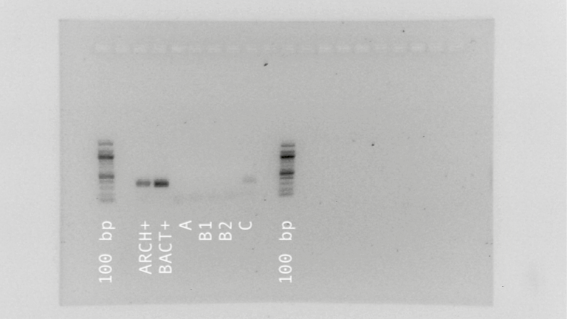
\includegraphics[width=\textwidth]{graphics/pic/20180130_EMP_OneTaq.png}
\end{figure}

Figure \ref{fig:20180130_EMP_OneTaq} shows the gel. The two positive controls confirms that reagents are fine. But it seems that there was no amplification DNA extracted with methods A, B2, B2, and there was a little amplification for DNA extracted with method C which is our usual extraction protocol. 

After discussing with Mia, she confirms that she resuspended the DNA pellet in TE buffer at the end of extraction methods A, B1, B2 (the TE buffer is provided in the kit).

\important{TE buffer contains \gls{edta} which chelates ions and therefore inhibits enzymatic activity which is good for long time storage of nucleic acid as \gls{edta} will inhibit DNase activity and therefore preserve the DNA. However, \gls{edta} also inhibit the DNA polymerase.}

Method C ends with the resuspension of the DNA pellet in Tris buffer. I will try to amplify these sample samples adding enhancers. Also, Mia was repeating the DNA extraction with the kit and she resuspended the pellet in Tris buffer. So hopefully we can amplify this DNA.

